                                                                                                                                                                                                                                                     \documentclass{article}
\usepackage{amsmath}
\usepackage{amsthm}
\usepackage{amssymb}
\usepackage{algorithm}
\usepackage{graphicx}
\usepackage[noend]{algpseudocode}

\newlength\tindent
\setlength{\tindent}{\parindent}
\setlength{\parindent}{0pt}
\renewcommand{\indent}{\hspace*{\tindent}}

\title{Manhattan Skyline Problem}
\author{Daniel Braithwaite}

\begin{document}
	\pagenumbering{gobble}
	\maketitle
	\newpage
  	\pagenumbering{arabic}
  	
	\section{Partitioning The Problem}
		There are two ways of partitioning the Manhattan Skyline problem, one is by partitioning the list of buildings e.g. breaking the list down the middle. The other option is to partition the x-axis.
	
		\subsection{Partitioning By Buildings}
			When dividing the problem by the list of buildings, splitting the problem up is easy. You keep dividing the problem in half until you only have one building, from here calculating the skyline for one building is trivial. However recombining the skylines from two different sets of buildings is where it gets tricky.
			
		\subsection{Partitioning By x-axis}
			Partitioning this way would make combining solutions easier as by the time you reach the base case you would have a solution for some $x$ value and combining would be trivial. The hard part would be the splitting, you would want to split between buildings and try to avoid splitting in the middle of the building as then you would have that building in two lists.
		
	\section{Algorithm}
		The algorithm I designed splits the problem down by breaking up the list of buildings, halving it each time, until a list of size 1 is reached, at which point constructing the skyline for a single building is trivial. Merging the skylines back together is a bit more complicated, it works by taking the two partial skylines and moving through them at each point taking the one with the smallest $x$, Say we choose the next element from the left skyline then we also need to look at the last added element from the right skyline so we could tell if the left skyline was dropping below the right.\newline\newline
		
		When designing my algorithm I could of separated the main loop into two so that if we reached the end of one skyline we could just append the the rest of the remaining list to the output skyline. However this wouldn't improve the efficiency of the algorithm. I also felt it was more elegant to have it all in one loop.\newline\newline
		
		
	
		\begin{algorithm}
			\begin{algorithmic}[1]
				\Procedure{recConstructSkyline}{$buildings,start,end$}
					\If{$end - start = 1$}
						\State $building \gets buildings[start]$
						\State
						\Return skyline for building
					\EndIf
					
					\State $middle \gets (end - start)/2$
					\State
					\Return $mergeSkylines(recConstructSkyline(buildings, start, middle+start), recConstructSkyline(buildings, middle+start, end))$
				\EndProcedure
				
				\State				
				
				\Procedure{mergeSkylines}{$leftSkyline, rightSkyline$}
					\State $skyline \gets empty list$
					\State
					\State $left \gets 0$, $right \gets 0$
					\State
					\While{$left < leftSkyline.size$ or $right < rightSkyline.size$}
						\If{$left >= leftSkyline.size$}
							\State $currentPair \gets rightSkyline[right]$
							\State $prevPair \gets leftSkyline[left-1]$
							\State $right++$
						\ElsIf{$right >= rightSkyline.size$}
							\State $currentPair \gets leftSkyline[left]$
							\State $prevPair \gets rightSkyline[right-1]$
							\State $left++$
						\ElsIf{$leftSkyline[left].x < rightSkyline[right].x$}
							\State $currentPair \gets leftSkyline[left]$
							\State $prevPair \gets rightSkyline[right-1]$ if possible
							\State $left++$
						\ElsIf{$rightSkyline[right].x < leftSkyline[left].x$}											\State $currentPair \gets rightSkyline[right]$
							\State $prevPair \gets leftSkyline[left-1]$ if possible
							\State $right++$
						\Else
							\State $currentPair \gets leftSkyline[left]$
							\State $prevPair \gets rightSkyline[right]$
							
							\State $right++$
							\State $left++$
						\EndIf
						\State
						\If{$prevPair$ is unassigned}
							\State add currentPair to skyline
							\State return to top of loop
						\ElsIf{$currentPair.height > prevPair.height$}
							\State skyline.add(currentPair)
						\Else
							\State $change \gets [currentPair.x, prePair.height]$
							
							\If{$skyline.lastElement.height != change.height$}
								\State skyline.add(change)
							\EndIf
						\EndIf  
					\EndWhile
				\EndProcedure
			\end{algorithmic}
		
		\end{algorithm}
		
		\break
		
	\section{Proof Of Correctness}

		\subsection{Assumption}
			\begin{enumerate}
				\item The input is a list of triples of the form $(x_1, x_2, height)$, where $x_1 < x_2$
			\end{enumerate}
		
		\subsection{Requirements}
			\begin{enumerate}
				\item Sorted in ascending order by $x$
				\item The height at any $x$ position is the maximum height of any building spanning that $x$
				\item Any change in height must occur at the start or end of a building $x$ 
			\end{enumerate}
		
		\subsection{Direct}
			There is only one building as $n = 1$ say we had the building $(x_1, x_2, h)$ the skyline is trivial to create, we get the following ${(x_1, h), (x_2, 0)}$. Therefor clearly the requirements hold.
			
			\begin{enumerate}
				\item As in the input $x_1 < x_2$ then the skyline is sorted
				\item There is only one building so we can clearly see this is true as for any $x_1 <= x <= x_2$ the height is that of the building
				\item By the way we constructed the skyline, part three must hold as the only times the height changes is at $x_1$ and $x_2$ and these two $x$ values are at the start and end of the building
			\end{enumerate}
			
		\subsection{Divide}
			When we are splitting the data we don't touch the triples so the assumption still holds\newline
			$n_i < n$ as we are splitting the list into two halves from the middle so $n_i = n/2 < n$\newline
			
		\subsection{Combine}
		
			\subsubsection{Requirement 1}
			First we show that the output skyline is sorted, showing that part 1 of the requirements is true for the out. To show this we will use a loop invariant.\newline
			
			\textbf{Loop Invariant}
			\begin{enumerate}
				\item Skyline is sorted
			\end{enumerate}				
			
			\textbf{Initialization:} Here $skyline \gets \varnothing$ and therefore is trivially sorted\newline
			
			\textbf{Maintenance:} We are choosing the next $x$ to be added from the left and right skylines, both of which are sorted. We look at the next element in both the lists and take the one with the smaller $x$ adding this to the skyline. so we can see if we have the skyline ${x_1, ....., x_k, x_{k+1}}$ then $ x_1 < ..... < x_k < x_{k+1})$.\newline
			
			Therefore part one of the requirements holds.
			
		
			\subsubsection{Requirement 2}
			Now we need to show that at any $x$ the height is the highest of any building at that $x$. We are merging two skylines, we will refer to these as the left and the right skylines.
			
			We start by looking at how we choose the next $x$ to be added to the skyline. When choosing this we look at the next element in the left and right skylines that are to be merged and pick the one with the smaller starting $x$. We set this to be currentPair.\newline
			
			Based on what list we choose currentPair from we set prevousPair to be the last element added to the output skyline from the other list. We are interested in this prevousPair because we want to keep track of the height in the other list so if the currentPair height drops below it then we know that the skyline is overlapping.\newline
			
			There are three cases
			\begin{enumerate}
				\item $currentPair.height > prevousPair.height$
				\item $currentPair.height < prevousPair.height$
				\item $currentPair.height = prevousPair.height$
			\end{enumerate}
			
			\textbf{Case 1} and \textbf{Case 3} are trivial, we just add the pair $(currentPair.x, currentPair.height)$ to the skyline\newline
			
			\textbf{Case 2} requires some more thought, we cant just add the pair $(currentPair.x, currentPair.height)$ as the height of the other skyline is still prevousPair.height. So we add the pair $(currentPair.x, previousPair.height)$.
			
			\subsubsection{Requirement 3}
				Requirement part 3 holds as the next $x$ to be added is chosen from ether the left or right skyline, we know that all the requirements hold for the left and right skylines so therefore any $x$ taken from them must be where a building starts or finishes.
	
	\section{Complexity}
	
		\subsection{Direct}
	
		The complexity of solving the direct solution is $O(1)$, when we have one building constructing the skyline is very simple its just two tuples. Constructing this is clearly is $O(1)$.\newline		
		
		\subsection{Divide}		
		
		The complexity of the divide part of the algorithm is also $O(1)$ as nothing actually happens here we just recursively pass the array of buildings with a section for the function to look at.\newline
		
		\subsection{Combining}		
		
		Combining has a complexity of $O(n)$ where n is the total number of buildings represented by the left and right skylines, we see this when we look at the following. The algorithm for merging skylines takes two skylines as input and will return one representing the combination. Each of the two input skylines represents $n/2$ buildings so at worse case (all the buildings being disjoint) each of the skylines will contain $2 * n/2 = n$ tuples. Meaning the loop will iterate at most $2n$ times. Thus giving us $O(n)$\newline
		
		\subsection{Asymptotic Cost}		
		
		So we want to solve the following recurrence relation using the master method we have\newline\newline
 
		\[ 
			T(n) = 
			\begin{cases}
				1 & n == 1\\
				2T(n/2) + n + 1 & otherwise
			\end{cases}
		\]\newline\newline
		
		We fit what we have to the following from the master method\newline
		\[
			T(n) = aT(n/b) + f(n)
		\]
		
		where we know that
		\[
			a = 2, b = 2, f(n) = n + 1
		\]
		
		so we let
		
		\[
			\alpha = \log_2 2 = 1
		\]		
			
		and we see that			
				
		\[
			f(n) \in \theta(n^1) = \theta(n)
		\]
		
		so finally by the master theorem we see that the asymptotic cost is the following 
		
		\[
			\theta(n\log_2 n)
		\]
		
	\section{Implementation}		
		
		When implementing the algorithm I used a list to store the buildings and to store the skylines. There can be a cost to adding to the list when the internal array gets full. We can get remove this cost as we know the maximum size of the new skyline so we can initialize the list with the maximum possible size. Using a list also meant it was very easy to divide up the buildings using indices without actually having to create any new lists.
		
	\break		
		
	\section{Testing}
	
		I tested my algorithm on a number of randomly generated test cases from size 10000 to 100000, the results where promising as they matched up perfectly with my theoretical complexity. At each input size there where three test cases. The steps plotted on the y-axis is the number of times the loop in the merge function executes for each of the problem instances as everything inside this loop was constant time so all we need to worry about is the number of times it executes\newline\newline

		\begin{enumerate}
			\item \textbf{Worst Case} where all the buildings are disjoint, i.e. none of them overlap
			\item \textbf{Average Case} where all the buildings are randomly distributed 
			\item \textbf{Best Case} where all the buildings overlap
		\end{enumerate}
		
		\begin{figure}[h]
			\vspace{3mm}
			\begin{center}
				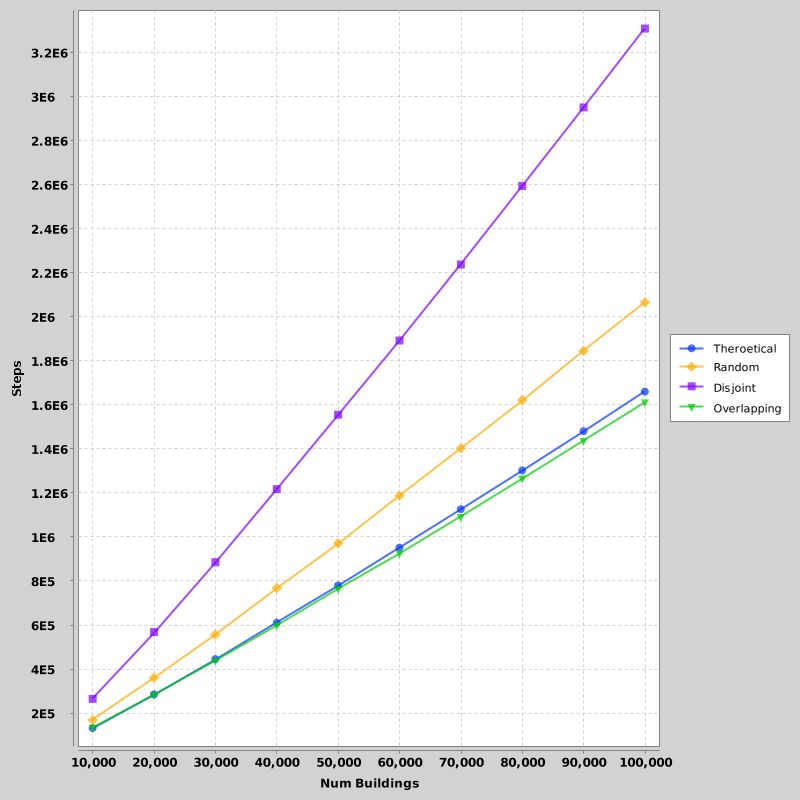
\includegraphics[scale=0.4]{data.png}
			\end{center}
		\end{figure}
		
		As you can see in the graph above the theoretical complexity is bounded from above by the worst case(purple line) and bounded from below by the best case (green line). This matches up with the theoretical complexity $nlog_2(n)$
  
\end{document}